\section{Status and Evaluation}
\label{sec:evaluation}

\subsection{Portability}
We have two partial, proof-of-concept implementations, one over UDP sockets and
one over Portals 3.3.

The socket prototype driver opens one SOCK\_DGRAM (UDP) socket per CCI endpoint
and has to provide reliability (acknowledgement and retransmission on loss).
The socket driver also has to multiplex connections over the single socket.
Enough functions are complete including RMA write to allow simple pingpong
tests to exercise the CCI API.

The Portals implementation also implements enough functions to run a pingpong
test with active messages. Since Portals assumes a reliable interconnect, the
only difference between a CCI UU connection and a RO/RU connection is that we
complete a UU send when we receive the Portals' SEND\_END event which indicates
that the sender's buffer is no longer needed (i.e. the data is on the wire).
For a reliable connection, we report a completion when we get the Portals' ACK
of receipt at the peer.

\subsection{Performance}
We wrote a native Portals pingpong and compared it to the CCI pingpong
performance. We ran tests on a Cray XT6 and locked the processes to the same
cores for both tests. The CCI over Portals \begin{math}\frac{1}{2}\end{math}RTT
was less than 200 ns more than the native Portals' performance up to 256 bytes.
For an eight byte message, for example, CCI's latency is 5.91 \us versus 5.74
\us for native Portals. Figures \ref{fig:latency} and \ref{fig:bw} show latency
and bandwidth for active messages up to 8 KB on a Cray XT6.

\begin{figure}[htbp]
\centering
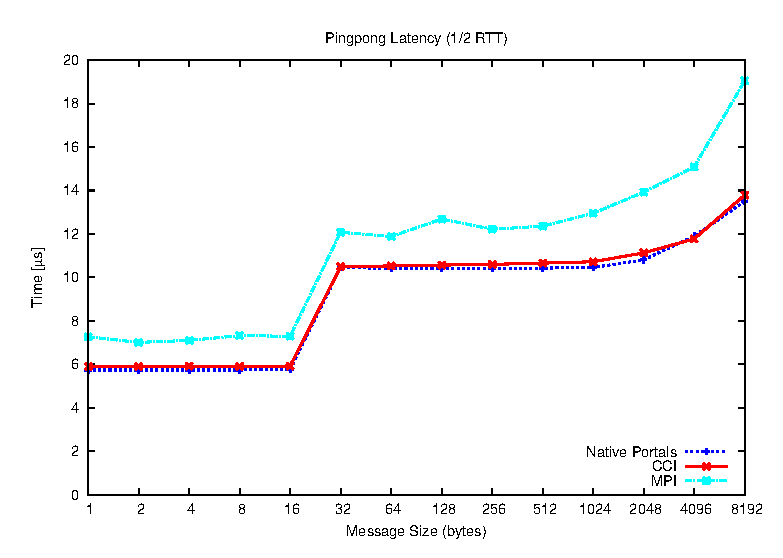
\includegraphics[width=3.45in]{pingpong-latency.eps}
\caption{Pingpong Latency when using Portals on SeaStar}
\label{fig:latency}
\end{figure}

\begin{figure}[htbp]
\centering
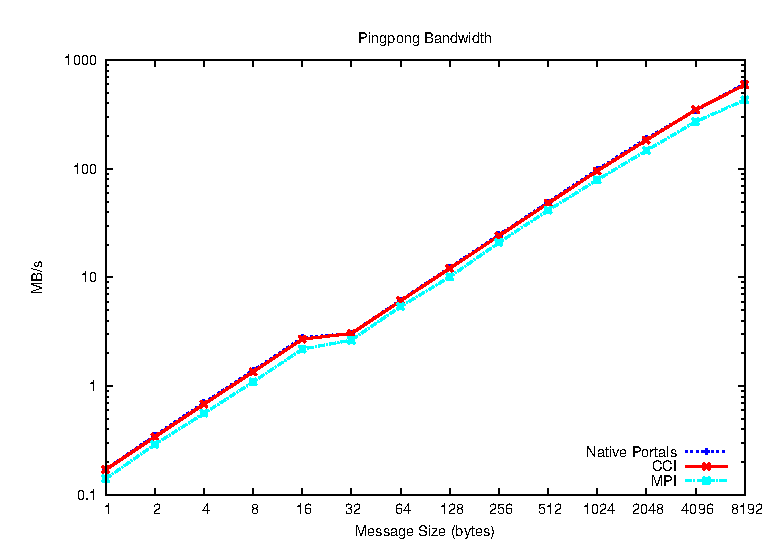
\includegraphics[width=3.45in]{pingpong-bw.eps}
\caption{Pingpong Bandwidth when using Portals on SeaStar}
\label{fig:bw}
\end{figure}

\begin{figure}[htbp]
\centering
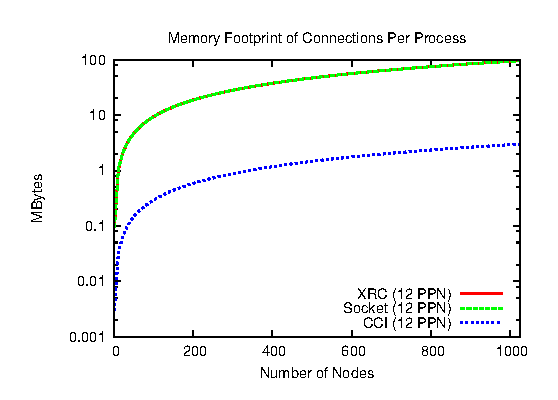
\includegraphics[width=3.45in]{memory_log.eps}
\caption{Memory footprint for connections per process}
\label{fig:memory}
\end{figure}

\subsection{Scalability}
CCI uses connection-oriented semantics with minimal per-connection resources.
For the Portals driver, each connection requires 104 bytes on 64-bit machines
(20 bytes for the public CCI connection struct, 20 bytes for the private CCI
struct, and 64 bytes for the Portals driver connection struct).  The sock driver
needs 140 bytes for each connection.

Figure \ref{fig:memory} shows the connection state (not including buffers) for
Verbs, sockets, and CCI. The memory usage for Verbs comes from
\cite{Shipman:2008:XIS:1431669.1431683} for X-SRQ which uses a single shared
receive QP for each node along with a send QP for each peer process. This is
the best case scenario for Verbs. Originally, Verbs required
\begin{math}O(N^2)\end{math} QPs. The sockets usage is derived from a single 4
KB page for send and receive buffers in addition to some minimal internal state.

The CCI usage conservatively assumes 256 bytes (assuming alingment padding,
etc.) as used in the UDP driver. Obviously, if CCI is implemented over Verbs,
for example, then this amount is on top of the underlying implementation. In
order to provide support for Verbs hardware (Infiniband, iWarp, etc.), we intend
to use Verb's Unreliable Datagram (UD) mode to avoid the QP memory usage by
Verb's Reliable Connected (RC) mode.


\subsection{Robustness}

